\documentclass[10pt,a4paper]{article}
\usepackage[utf8]{inputenc}
\usepackage[spanish]{babel}
\usepackage{amsmath}
\usepackage{amsfonts}
\usepackage{amssymb}
\usepackage{graphicx}
\author{Erick de Jesus Hernández Cerecedo}
\title{Resumen del texto Modelos de Calidad del Software, un estado del arte}
\begin{document}
\maketitle

\section{Introducci\'on}
El software es una de las herramientas de mayor utilidad en la optimizaci\'on de los procesos en las empresas, con el fin de consegir eficiencia y satisfacer las necesidades de los usuarios, raz\'on por la cual el software debe contar con criterios que garantizen su calidad. Existen diversas metodolog\'ias, estandares de calidad, guias y normas propuestas con el fin de evaluar la calidad del mismo.

\begin{enumerate}
	\renewcommand{\theenumi}{\Roman{enumi}}
	\item Contextualizacion de calidad de software
		\begin{list}{}{}
			\item El t\'ermino calidad de software se refiere al desempeño de las principales caracter\'isticas con las que debe cumplir un sistema computacional durante su ciclo de vida, este brinda confiabilidad y aumenta la sitisfacci\'on de clientes. El concepto de calidad de sofware seg\'un Pressman (2010) se asocia a la ``concordancia con los requisitos funcionales y de rendimiento expl\'icitamente establecidos con los est\'andares de desarrollo plenamente documentados y con las carcater\'isticas implicitas que se espera de todo software desarrollado profesionalmete", denotando que el \'enfasis radica en los requisitos especificos del sistema y en la busqueda de satisfacci\'on del cliente.
		\end{list}
	\item Modelos de calidad de software
		\begin{list}{}{}
			\item Segun Scalone, 2006 ``los modelos de calidad son aquellos documentos que integran la mayor parte de las mejores pr\'acticas, proponen temas de administraci\'on en los que 	cada organizaci\'on debe hacer \'enfasis, integran diferentes pr\'acticas dirigidas a los proyectos clave y permiten medir los avances en calidad''.
			Esta definici\'on dirigida a calidad, se identifican procesos que como soporte al mismo tiempo lleve documentaci\'on, y se valga de distintas pr\'acticas definidas en el modelo, con el fin de lograr una mejora continua, ser m\'as competentes, para poder medir la calidad y brindar productos o servicios de alto nivel.
			En el ambito de contrucci\'on el modelo de calidad debe permitir evaluar el sistema de forma cualitativa o cuantitativa, con el fin de proponer estrategias que permitan la mejora del proceso dentro de las etapas de an\'alisis, dise\~no, desarrollo y pruebas de software.
		\end{list}
	\item Estructura y enfoque de los modelos de calidad de software
	\begin{figure}[h]
		\centering 
		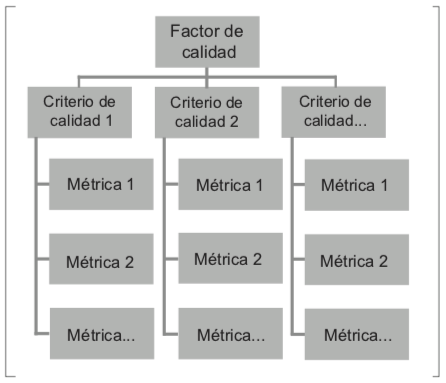
\includegraphics[width=0.8\linewidth]{estructuraSF.png}
		\caption{Estructura de calidad de software}
	\end{figure}
		\begin{list}{}{}
			\item Los modelos de calidad de software se clasifican de acuerdo con el enfoque de evaluaci\'on, ya sea a nivel proceso, producto o calidad en uso.
			\item \textbf{Calidad a nivel deproceso}
			\item La calidad de un sistema software debe ser programada desde el inicio del proyecto, y posteriormente en cada etapa del proceso de desarrollo, debe ser monitoreada para controlar los aspectos de calidad, minimizar los riesgos y ofrecer soporte continuo.
			\item \textbf{Calidad a nivel producto}
			\item Se refiere a especificar y evaluar el cumplimieto de criterios del producto, por esta raz\'on, algunas normas y \'estandares han definido la calidad a nivel producto en tres tipos:
				\begin{itemize}
					\item Interna
					\item Externa
					\item En uso
				\end{itemize}
			\item \textbf{Calidad en uso}
				\begin{figure}[h]
					\centering 
					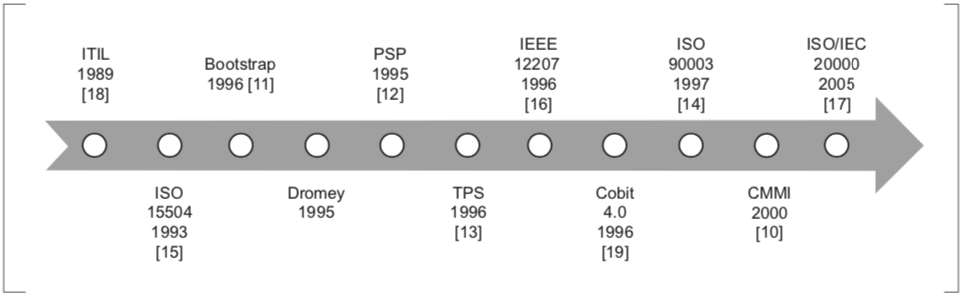
\includegraphics[width=1\linewidth]{nivel_proceso}
					\caption{L\'inea de tiempo de modelos a nivel proceso}
				\end{figure}
			\item La calidad de uso se define como ``El conjunto de atributos relacionados con la aceptaci\'on por parte del usuario final y seguridad''
			\item \textbf{\textit{Modelos a nivel proceso}}
				\begin{itemize}
					\item \textbf{ITIL}
					\item \textbf{ISO/IEC I5504}
					\item\textbf{ ISO/IEC I5504}
					\item \textbf{Bootstrap}
					\item \textbf{Dromey}
					\item \textbf{Personal Software Process (PSP)}
					\item \textbf{Team Software Process (TSP)}
					\item \textbf{IEEE / EIA 12207}
					\item \textbf{Cobit 4.0}
					\item \textbf{ISO 90003}
					\item \textbf{CMMI (Capability Maturity Model Integration)}
					\item \textbf{ISO / IEC 20000}
				\end{itemize}
			\item \textbf{\textit{Modelos a nivel producto}}
				\begin{figure}[h]
					\centering 
					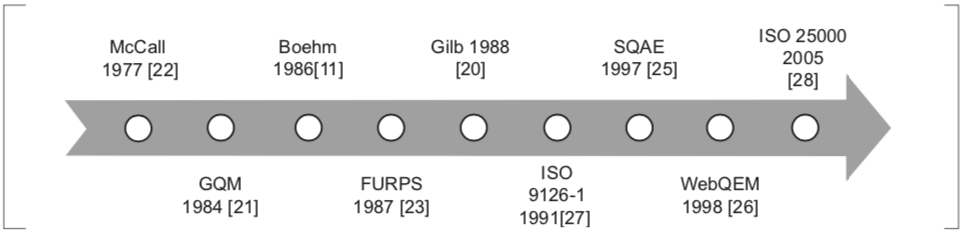
\includegraphics[width=1\linewidth]{nivel_producto}
					\caption{Modelos de calidad a nivel de producto}
				\end{figure}
				\begin{itemize}
					\item \textbf{McCall}
					\item \textbf{GQM o Goal Question Metric}
					\item \textbf{Boehm}
					\item \textbf{FURPS}
					\item \textbf{GILB}
					\item \textbf{ISO 9126}
					\item \textbf{SQAE o Software Quality Assessment Exercise}
					\item \textbf{WebQEM}
					\item \textbf{ISO 25000}					
				\end{itemize}
		\end{list}
	\item Experiencias de implementaci\'on de modelos de calidad de softwar
		\begin{list}{}{}
			\item Estas son algunas experiencias de aplicaci\'on de modelos y est\'andares de calidad de software. 
			\item \textbf{CMMI}
			\item \textbf{Bootstrap}
			\item \textbf{PSP Personal Software Process}
			\item \textbf{TSP Team Software Process}
			\item \textbf{ISO 90003}
			\item \textbf{ISO 15504}
			\item \textbf{ISO / IEC 20000}
			\item \textbf{ITIL}
			\item \textbf{COBIT 4.0}
			\item \textbf{GILB}
			\item \textbf{GQM}
			\item \textbf{McCall}
			\item \textbf{CMMI}
			\item \textbf{FURPS}
			\item \textbf{BOEHM}
			\item \textbf{DROMEY}
			\item \textbf{ISO 9126}
			\item \textbf{SQAE, ISO25000}
		\end{list}
\end{enumerate}





\end{document}